% !TEX root = Stanfill_CoDA.tex
\section{Results}\label{sec:results}

In this section we summarize and present the main findings of the simulation study for  estimating the central direction $\bm S = \bm I_{3\times 3}$ with the four proposed estimators of Section~\ref{sec:estimators}. We quantify the estimation error between the true location $\bm S = \bm I_{3\times 3}$ and an estimate $\widehat{\bm S}$ using the geodesic distance, i.e.
\begin{equation}
\Rdist(\bm{S}, \widehat{\bm{S}}) =  \frac{1}{\sqrt{2}}||
\Log(\bm{S}^\top\widehat{\bm{S}})||_F, \quad \mbox{where} \quad \widehat{\bm{S}} =  \ProjMean, \; \GeomMean,\;  \ProjMedian \; \mbox{or} \; \GeomMedian.
\end{equation}

\noindent Results using $\Edist$ would prove equivalent, albeit on a smaller scale as noted in Section~\ref{subsec:metrics}.   
%\begin{center}
\begin{figure}[h!]
\centering
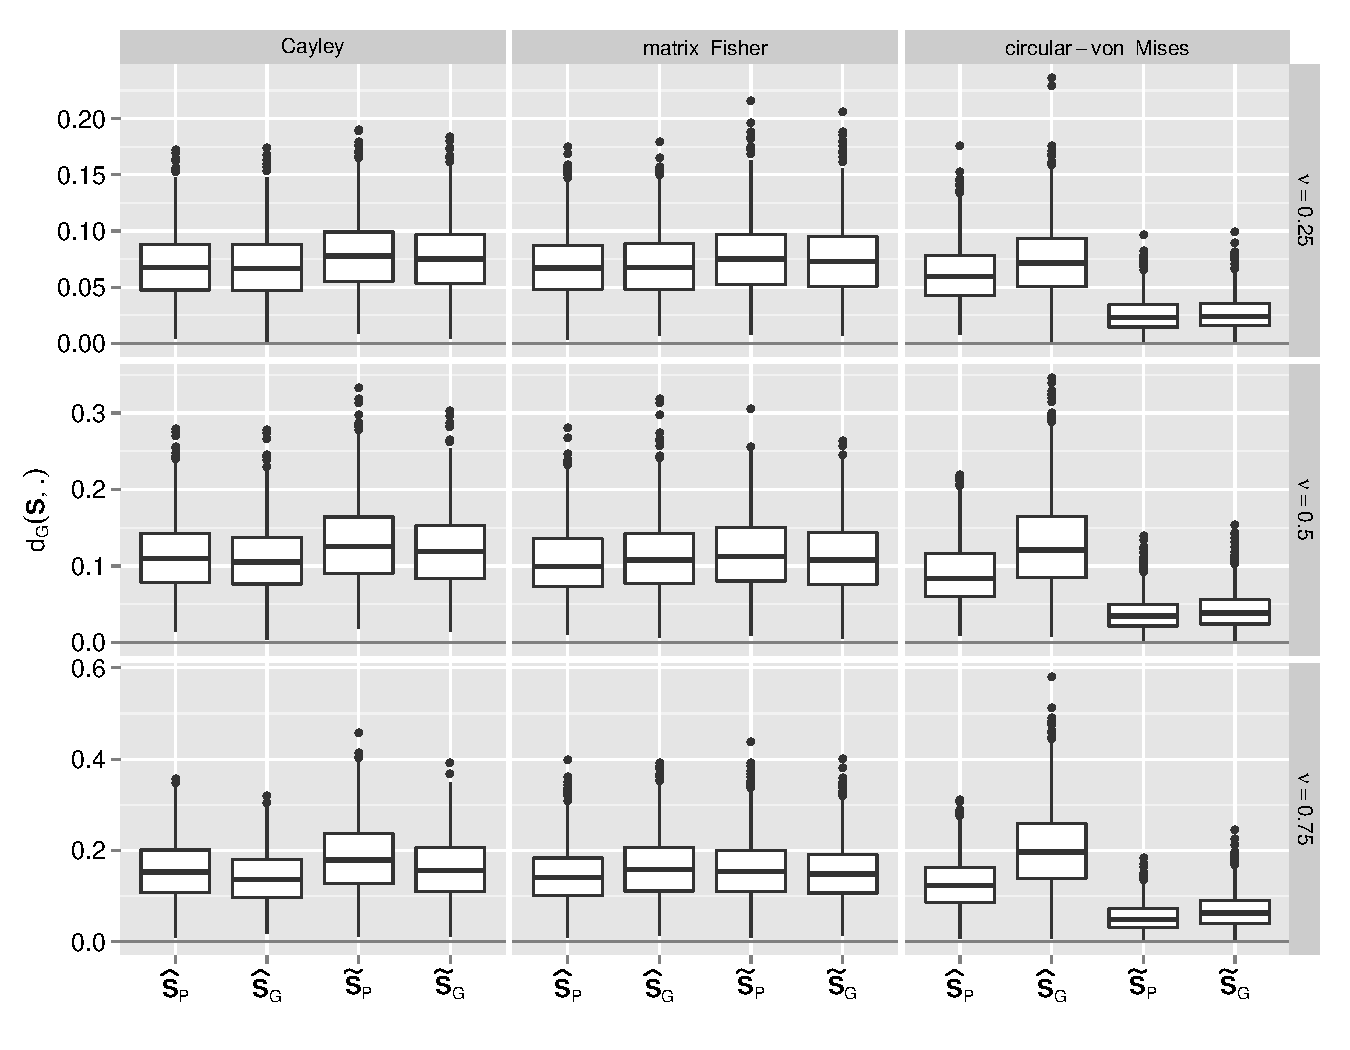
\includegraphics[width=0.8\textwidth]{N100AllNuBoxes.pdf}
\caption{Boxplots of the estimation errors for each rotation distribution and level of $\nu$,  $n=100$.}
\label{fig:NuBoxes}
\end{figure}
%\end{center}
Figure~\ref{fig:NuBoxes} displays side-by-side boxplots showing the estimation errors of all four estimators for a given choice of rotation distribution and circular spread $\nu$ when  $n=100$.   For a tabular summary of this figure including the root mean square error (RMSE)  as well as the \textit{mean estimation error} and estimated standard errors we refer to Table 5 in the online supplement. 

First and foremost the results suggest that different location estimators emerge as preferable depending on the type of distribution assumed for the rotation errors in \eqref{eqn:1}.  For the circular-von Mises-based distribution both median-type estimators ($\ProjMedian$ and $\GeomMedian$) are superior with respect to the estimation error while for the Cayley and matrix Fisher models the mean-type estimators ($\ProjMean$ and $\GeomMean$) perform slightly better though on a less pronounced scale.   Figure~\ref{fig:NuBoxes} further shows that the estimation error is a function of the circular spread $\nu$; as $\nu$ decreases the range of the observed estimation errors decreases within each rotation model and for each of the four estimators. The same holds for the mean estimation error and RMSE.  Similarly, the estimation error decreases as the sample size $n$ increases. This result is shown in Figure 11 in the online supplement.

While preferences within the median- and mean-type estimators are visible, these generally disappear as the variability in the data, i.e.~$\nu$ decreases.  For the Cayley and the matrix Fisher distribution the overall pattern of estimation is similar. $\ProjMean$ and $\GeomMean$ typically exhibit less spread and a lower average estimation error than $\ProjMedian$ and $\GeomMedian$ with differences between the estimators lessening as $\nu$ becomes smaller.

Figure~\ref{fig:vmnu75} illustrates the extent to which the mean estimation error and RMSE as a function of sample size differ with respect to estimator choice for the circular-von Mises-based distribution when $\nu=0.75$.  We can see more clearly the advantage of the median estimators over the mean estimators across sample sizes.
 \vspace{-1em}\begin{figure}[h!]
\centering
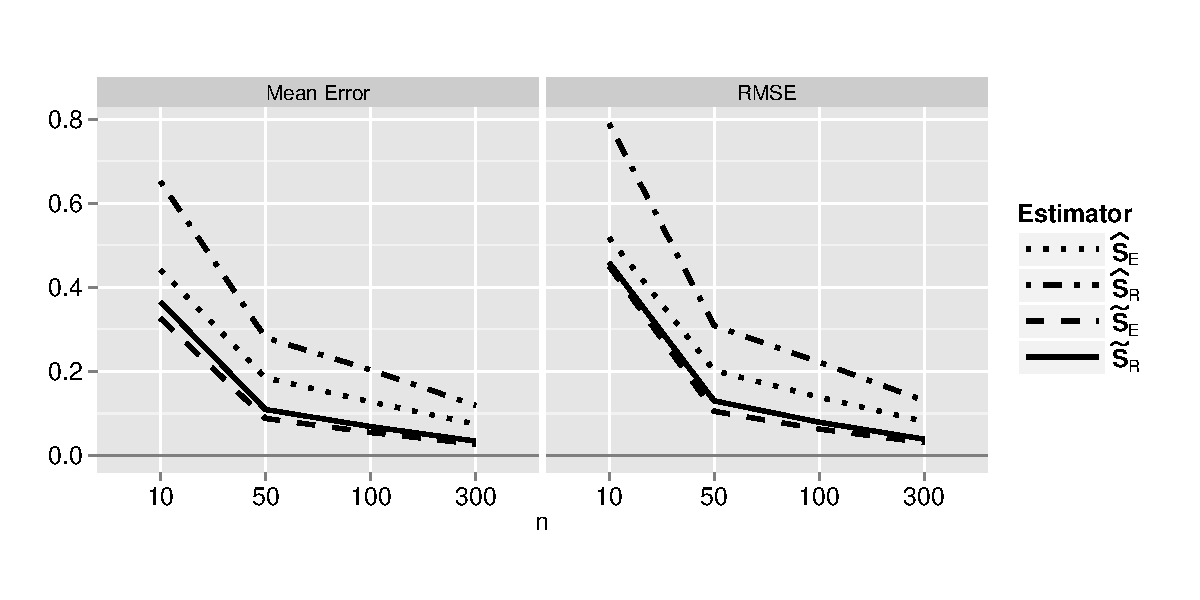
\includegraphics[width=0.8\linewidth]{vonMisesnu75MeanRMSE.pdf}\vspace{-1em}
\caption{Plot of the estimation error for all levels of $n$ for the circular-von Mises-based distribution,  $\nu=0.75$.}  \label{fig:vmnu75}
\end{figure}\vspace{-1em}

The previous findings raise the question why, unlike the Cayley and the Fisher matrix distribution, the circular-von Mises-based distribution so clearly distinguishes between the mean- and median-type estimators. A first insight can be obtained from Figures~\ref{fig:Haar} (b) and (c) which reveal that out of the three distributions the circular-von Mises-based distribution exhibits the heaviest tail. Thus, we can expect a larger proportion of   \textit{more extreme} observations to be sampled under the circular-von Mises-based distribution suggesting that a median-type estimator is more favorable. 
We use Figure \ref{fig:SimTail} to examine the extent to which the tail-behavior indeed accounts for the observed differences in the mean- and median-type estimators. Figure \ref{fig:SimTail} displays for each simulated sample of size $n=300$ the proportion of observations in the sample considered to come from the tail of the distribution plotted against the difference in errors for the mean- and median-type estimators.  The results shown in Figure \ref{fig:SimTail} are with respect to the Euclidean geometry-based estimators $\ProjMean$ and $\ProjMedian$. Similar results are obtained for the Riemannian geometry-based estimators $\GeomMean$ and $\GeomMedian$ and therefore are omitted. Note that we define the tail to begin at the location obtained by averaging the three pairwise crossing points in Figure~\ref{fig:denzoom} at which the densities cross for the second time. From Figure \ref{fig:SimTail} we can see that with an increase in the proportion of tail observations the error of the mean estimator indeed increases at a higher rate than does the error of the median estimator, i.e.~the relative difference in the errors plotted on the $y$-axis increases. As a result the projected median is preferable to the projected mean more often as the tail becomes heavier. 
\begin{figure}[h!]
\centering
\vspace{-0.5cm}
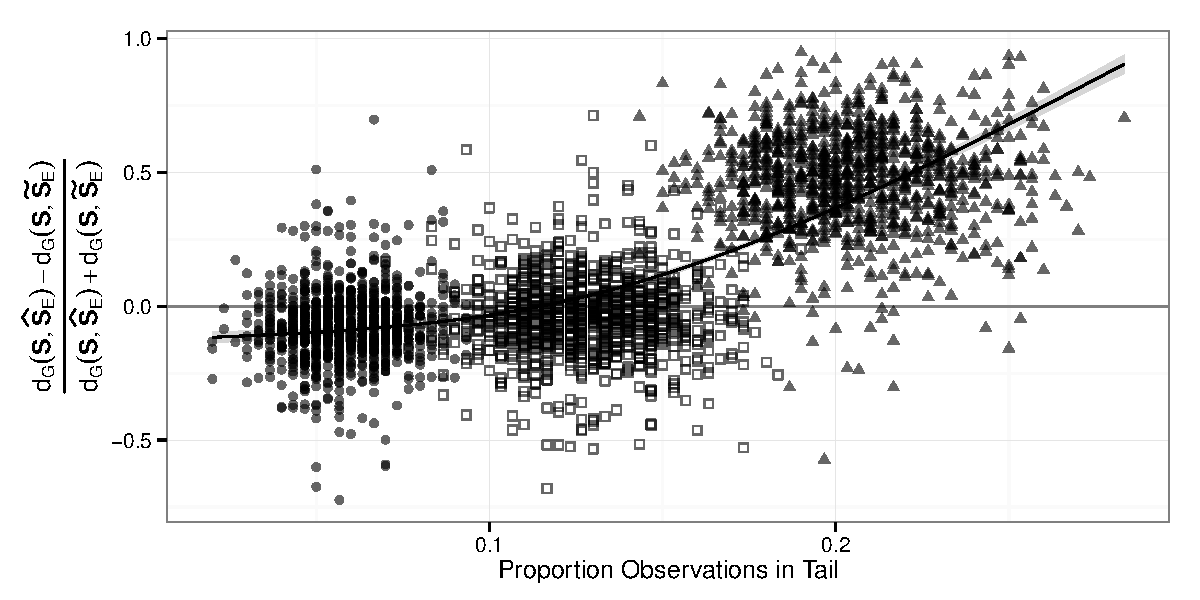
\includegraphics[width=.8\textwidth]{Nu75N300TailBehaviorStandard}
\caption{The proportion of observations in the tail against the difference in projected mean and median errors for simulated data with $n=300$.  Different symbols indicate different error distributions.}
\label{fig:SimTail}
\end{figure}

We next explore how the choice of geometric distance (Euclidean $\Edist$ or Riemannian $\Rdist$) affects the estimation error for both types of loss functions (i.e., $L_2-$norm or $L_1-$norm yielding a mean- or median type estimator, respectively). To provide more insight into the observed differences we plot in Figure~\ref{fig:comPL2} on the $x$-axis, for each type of loss function,  the estimation errors resulting from using $\Edist$ versus the corresponding estimation errors resulting from using $\Rdist$ ($y$-axis) for $n=100$ and $\nu=.25$,  $\nu=.75$, respectively.  That is, Figure~\ref{fig:comPL2} plots estimation errors in pairs (error with $\ProjMean$, error with $\GeomMean$) and (error with $\ProjMedian$, error with $\GeomMedian$). Paired estimators based on the $L_2-$norm ($\ProjMean, \GeomMean$) are represented by black dots whereas the $L_1-$norm ($\ProjMedian, \GeomMedian$) based estimators correspond to light gray dots. For example, Figure \ref{fig:comPL2} suggests that  $\GeomMedian$ tends to yield less estimation error than $\ProjMedian$  for the Cayley distribution as most of the points fall below the identity line while the Riemannian distance-based estimators $\GeomMedian$ and $\GeomMean$ result in greater errors for ${\bm S}$ than their Euclidean distance based counterparts for the circular-von Mises-based distribution. These findings support similar results for $\ProjMedian$ and $\GeomMedian$ seen earlier in Figure~\ref{fig:NuBoxes}.
\begin{figure}[h!]
\centering
\subfloat{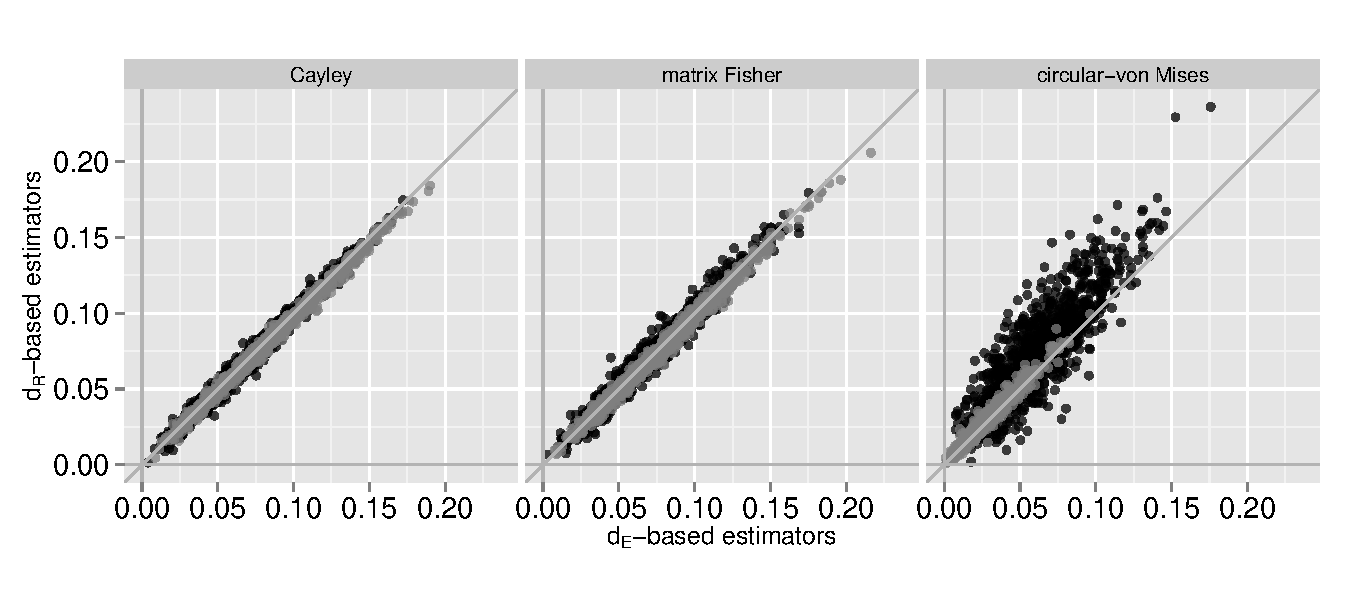
\includegraphics[width=0.8\linewidth]{EuclidRiemannNu25.pdf}}\\
\subfloat{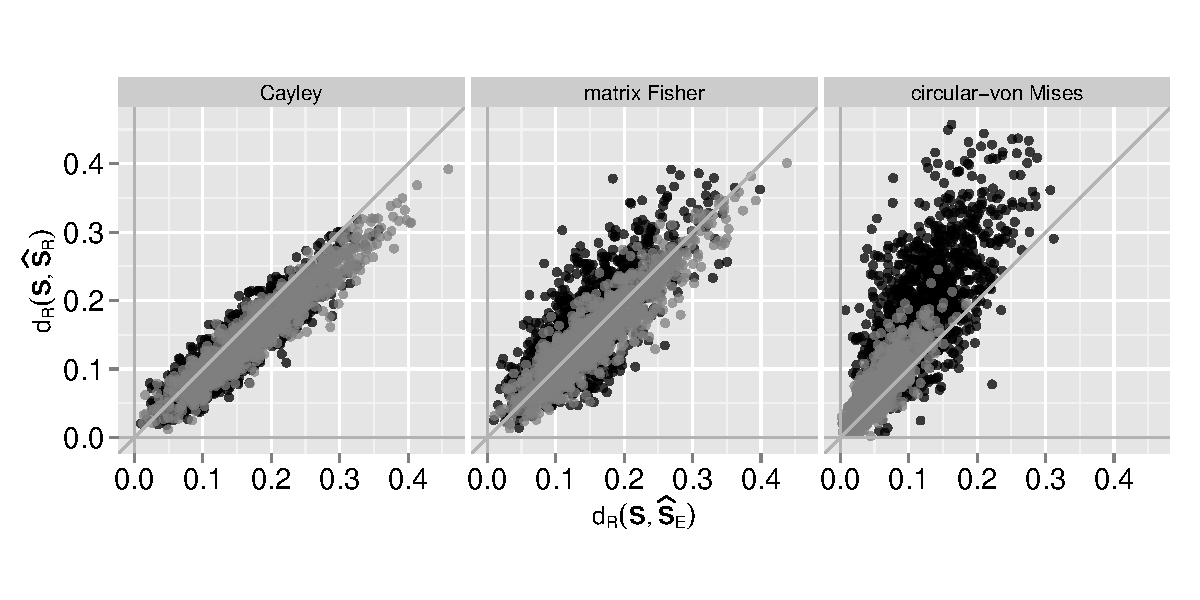
\includegraphics[width=0.8\linewidth]{EuclidRiemannNu75.pdf}}
\caption{Comparison of the estimation errors resulting from $\Edist$ ($x$-axis) and $\Rdist$ ($y$-axis) approaches based on simulated random samples of rotations with $n=100$.  Dots in black are estimation error pairs from $L_2-$norm based estimators, light gray dots denote estimation error pairs for $L_1-$norm based estimators.}
\label{fig:comPL2}
\end{figure}
Tables 3 and 4 of the online supplement support Figure~\ref{fig:comPL2} with an exact count (expressed as a percentage) of how often $\Rdist$ resulted in a smaller estimation error than $\Edist$.  Additionally, we show the average amount of error by which the Riemannian $\Rdist-$ and Euclidean $\Edist-$based estimates deviate from one another.   
Earlier results suggested the use of median-type estimators for the circular-von Mises-based distribution. Taking the findings with respect to the choice of geometry into account, we consider $\ProjMedian$ preferable for the circular-von Mises-based distribution as $\Rdist(\ProjMedian,\bm S) < \Rdist(\GeomMedian,\bm S)$ most of the time.  For the Cayley distribution our preference regarding the geometry is reversed; although differences are subtle $\Rdist$ is the preferred metric for the Cayley distribution especially when $\nu$ is large and overall $\GeomMean$ typically exhibits the least spread for this distribution.   For the  matrix Fisher distribution the preference is less clear, especially for less variable data, but as $\nu$ increases the Euclidean-based mean yields generally a smaller estimation error more often. In summary,
\begin{itemize}
\item the choice of location estimator can depend on the rotation error distribution in the location model (1).  For the matrix Fisher and the Cayley distribution  the projected arithmetic mean $\ProjMean$ and the geometric mean $\GeomMean$ are, respectively, preferable though $\ProjMedian$ and $\GeomMedian$ are not far behind especially when the circular spread is smaller. For the circular-von Mises-based distribution  the projected median $\ProjMedian$  should be used.

\item   a significant finding of the simulation results is that the (Euclidean-based)  projected median $\ProjMedian$ is typically a good location estimator across rotation error models.  For the circular-von Mises-based estimation, this generally has the best performance, while for the Cayley or matrix Fisher distributions, this estimator is often quite comparable to the best estimator.  In other words, $\ProjMedian$, an estimator  not previously considered for rotation matrices in the literature, appears to be suggestible, particularly in small samples and without knowledge of the underlying rotation error distribution.

%=======
%% !TEX root = Stanfill_CoDA.tex
%\section{Results}\label{sec:results}
%
%In this section we summarize and present the main findings of the simulation study for  estimating the central direction $\bm S = \bm I_{3\times 3}$ with the four proposed estimators of Section~\ref{sec:estimators}. We quantify the estimation error between the true location $\bm S = \bm I_{3\times 3}$ and an estimate $\widehat{\bm S}$ using the geodesic distance, i.e.
%\begin{equation}
%\Rdist(\bm{S}, \widehat{\bm{S}}) =  \frac{1}{\sqrt{2}}||
%\Log(\bm{S}^\top\widehat{\bm{S}})||_F, \quad \mbox{where} \quad \widehat{\bm{S}} =  \ProjMean, \; \GeomMean,\;  \ProjMedian \; \mbox{or} \; \GeomMedian.
%\end{equation}
%
%Results using $\Edist$ would prove equivalent, albeit on a smaller scale as noted in Section~\ref{subsec:metrics}.   
%%\begin{center}
%\begin{figure}[h!]
%\centering
%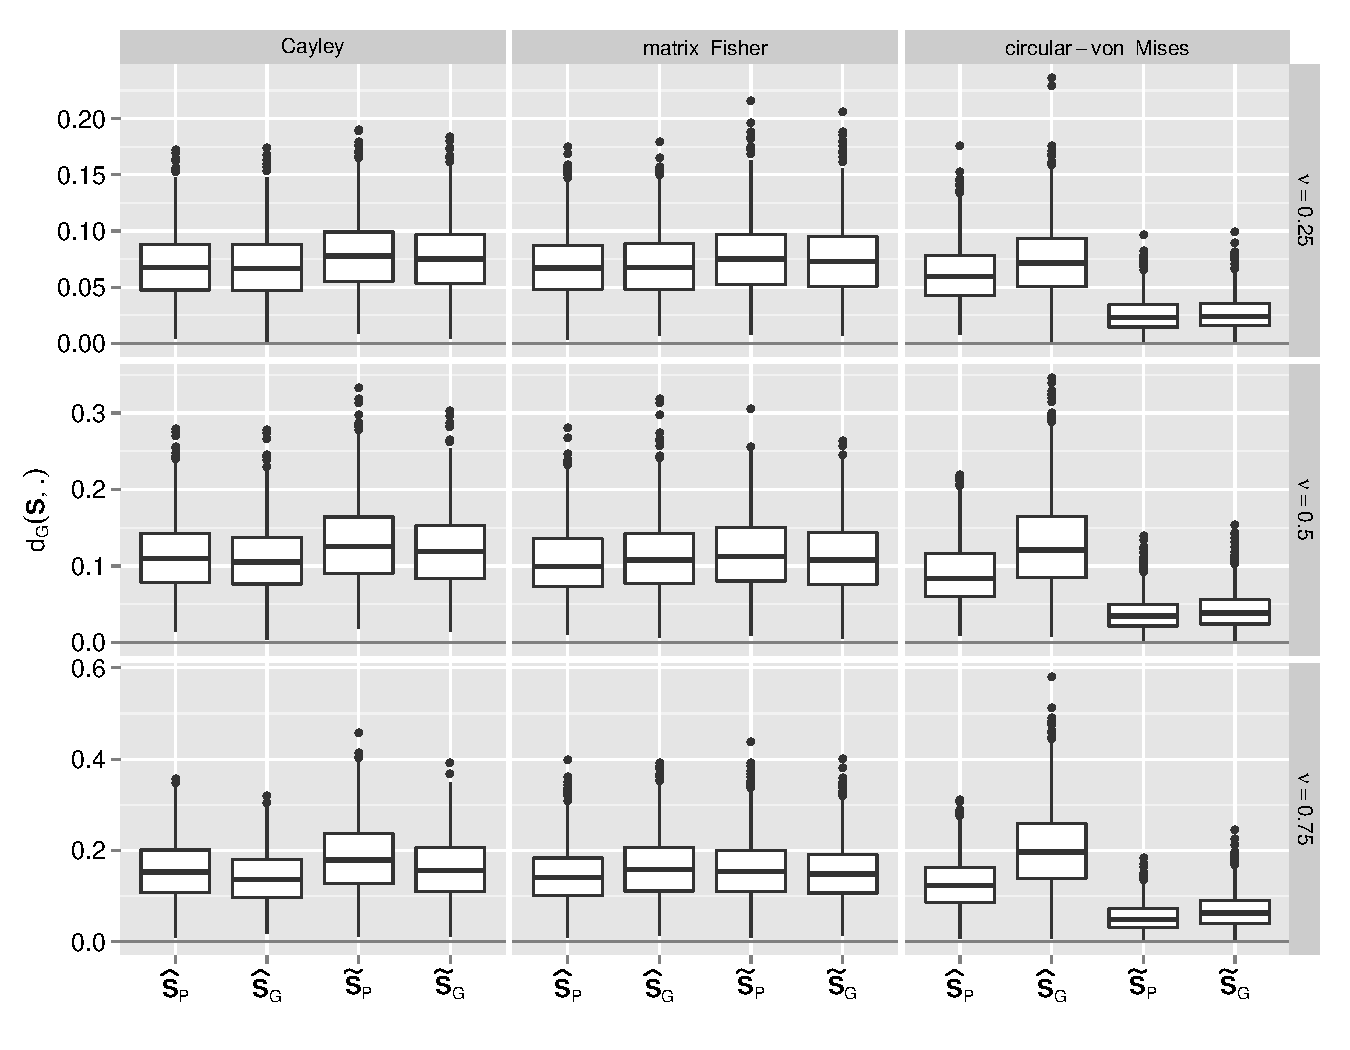
\includegraphics[width=0.8\textwidth]{N100AllNuBoxes.pdf}
%\caption{Boxplots of the estimation errors for each rotation distribution and level of $\nu$,  $n=100$.}
%\label{fig:NuBoxes}
%\end{figure}
%%\end{center}
%Figure~\ref{fig:NuBoxes} displays side-by-side boxplots showing the estimation errors of all four estimators for a given choice of rotation distribution and circular spread $\nu$ when  $n=100$.   For a tabular summary of this figure including the root mean square error (RMSE)  as well as the \textit{mean estimation error} and estimated standard errors we refer to Table 5 in the online supplement. 
%
%First and foremost the results suggest that different location estimators emerge as preferable depending on the type of distribution assumed for the rotation errors in \eqref{eqn:1}.  For the circular-von Mises-based distribution both median-type estimators ($\ProjMedian$ and $\GeomMedian$) are superior with respect to the estimation error while for the Cayley and matrix Fisher models the mean-type estimators ($\ProjMean$ and $\GeomMean$) perform slightly better though on a less pronounced scale.   Figure~\ref{fig:NuBoxes} further shows that the estimation error is a function of the circular spread $\nu$; as $\nu$ decreases the range of the observed estimation errors decreases within each rotation model and for each of the four estimators. The same holds for the mean estimation error and RMSE.  Similarly, the estimation error decreases as the sample size $n$ increases. This result is shown in Figure 11 in the online supplement.
%
%While preferences within the median- and mean-type estimators are visible, these generally disappear as the variability in the data, i.e.~$\nu$ decreases.  For the Cayley and the matrix Fisher distribution the overall pattern of estimation is similar. $\ProjMean$ and $\GeomMean$ typically exhibit less spread and a lower average estimation error than $\ProjMedian$ and $\GeomMedian$ with differences between the estimators lessening as $\nu$ becomes smaller.
%
%Figure~\ref{fig:vmnu75} illustrates the extent to which the mean estimation error and RMSE as a function of sample size differ with respect to estimator choice for the circular-von Mises-based distribution when $\nu=0.75$.  We can see more clearly the advantage of the median estimators over the mean estimators across sample sizes.
% \vspace{-1em}\begin{figure}[h!]
%\centering
%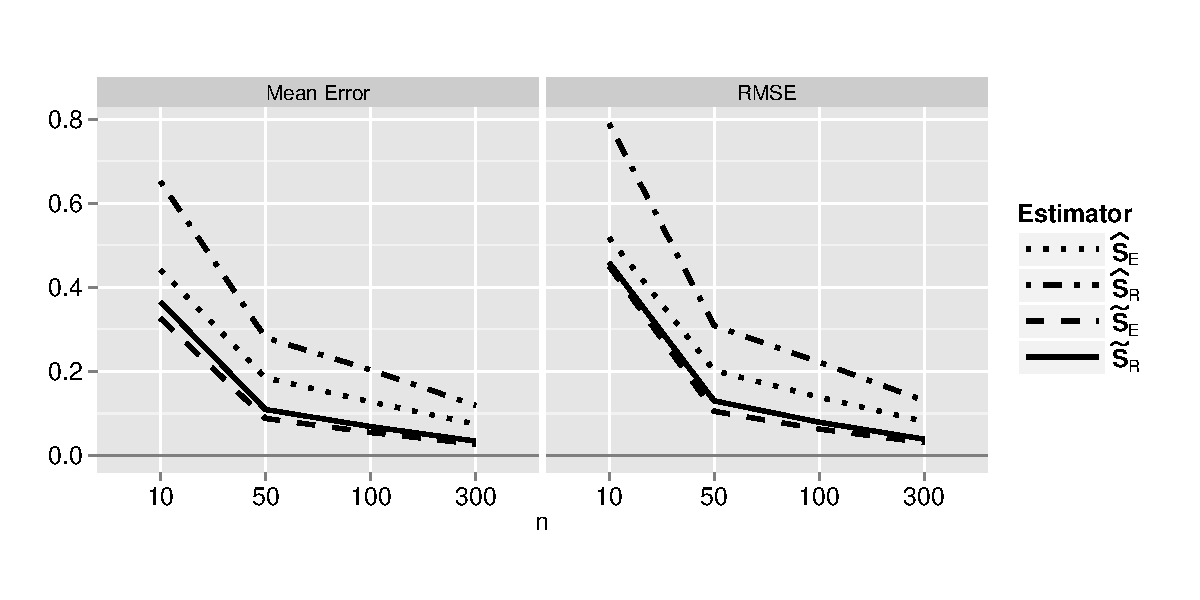
\includegraphics[width=0.8\linewidth]{vonMisesnu75MeanRMSE.pdf}\vspace{-1em}
%\caption{Plot of the estimation error for all levels of $n$ for the circular-von Mises-based distribution,  $\nu=0.75$.}  \label{fig:vmnu75}
%\end{figure}\vspace{-1em}
%The previous findings raise the question why, unlike the Cayley and the Fisher matrix distribution, the circular-von Mises-based distribution so clearly distinguishes between the mean- and median-type estimators. A first insight can be obtained from Figures~\ref{fig:Haar} (b) and (c) which reveal that out of the three distributions the circular-von Mises-based distribution exhibits the heaviest tail. Thus, we can expect a larger proportion of   \textit{more extreme} observations to be sampled under the circular-von Mises-based distribution suggesting that a median-type estimator is more favorable. 
%We use Figure \ref{fig:SimTail} to examine the extent to which the tail-behavior indeed accounts for the observed differences in the mean- and median-type estimators. Figure \ref{fig:SimTail} displays for each sample the proportion of observations in the sample considered to come from the tail of the distribution plotted against the difference in errors for the mean- and median-type estimators.  The results shown in Figure \ref{fig:SimTail} are with respect to the Euclidean geometry-based estimators $\ProjMean$ and $\ProjMedian$. Similar results are obtained for the Riemannian geometry-based estimators $\GeomMean$ and $\GeomMedian$ and therefore are omitted. Note that we define the tail to be the average crossing point at which the distributions cross for the second time, see Figure~\ref{fig:denzoom}. From  Figure \ref{fig:SimTail} we can see that with an increase in the proportion of tail observations the error of the mean estimator indeed increases at a higher rate than does the error of the median estimator, i.e.~the relative difference in the errors plotted on the $y$-axis increases. As a result the projected median is preferable to the projected mean more often as the tail becomes heavier.  \\
%\begin{figure}[h!]
%\centering
%\vspace{-0.5cm}
%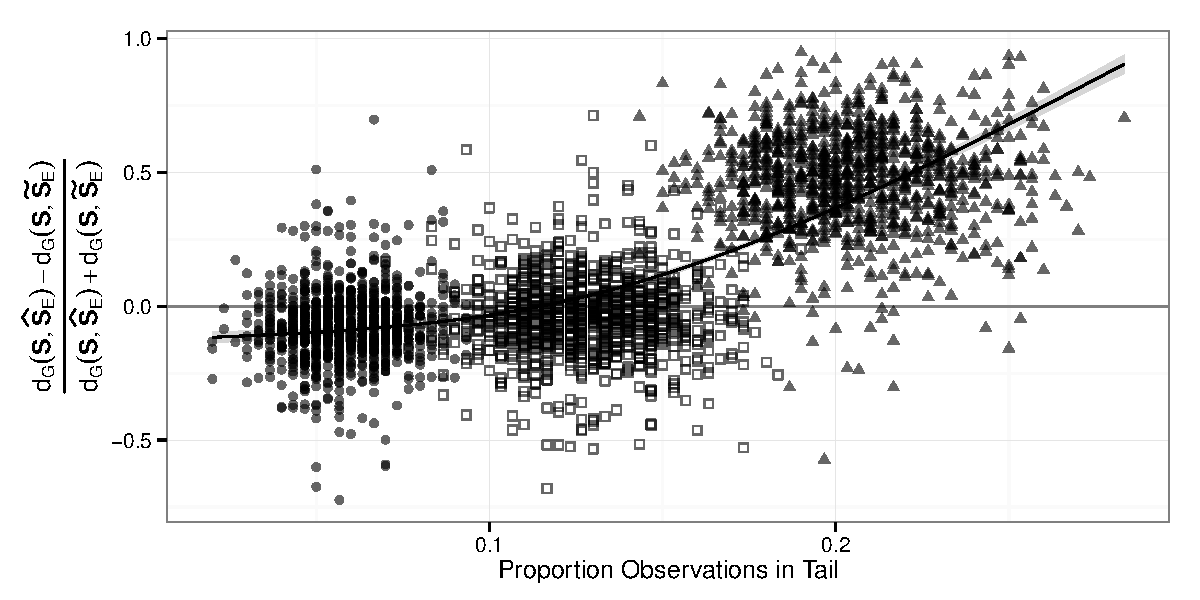
\includegraphics[width=.8\textwidth]{Nu75N300TailBehaviorStandard}
%\caption{The proportion of observations in the tail against the difference in projected mean and median errors for simulated data with $n=300$.  Different symbols indicate different error distributions.}
%\label{fig:SimTail}
%\end{figure}
%
%We next explore how the choice of geometric distance (Euclidean $\Edist$ or Riemannian $\Rdist$) affects the estimation error for both types of loss functions (i.e., $L_2-$norm or $L_1-$norm yielding a mean- or median type estimator, respectively). To provide more insight into the observed differences we plot in Figure~\ref{fig:comPL2} on the $x$-axis for each type of loss function  the estimation errors resulting from using $\Edist$ versus the corresponding estimation errors resulting from using $\Rdist$ ($y$-axis) for $n=100$ and $\nu=.25$,  $\nu=.75$, respectively.   Estimators based on the $L_2-$norm  are represented by black dots whereas the $L_1-$norm based estimators correspond to light gray dots. For example, Figure \ref{fig:comPL2} suggests that  $\GeomMedian$ tends to yield less estimation error than $\ProjMedian$  for the Cayley distribution as most of the points fall below the identity line while the Riemannian distance-based estimators $\GeomMedian$ and $\GeomMean$ result in greater errors for ${\bm S}$ than their Euclidean distance based counterparts for the circular-von Mises-based distribution. These findings support similar results for $\ProjMedian$ and $\GeomMedian$ seen earlier in Figure~\ref{fig:NuBoxes}.
%\begin{figure}[h!]
%\centering
%\subfloat{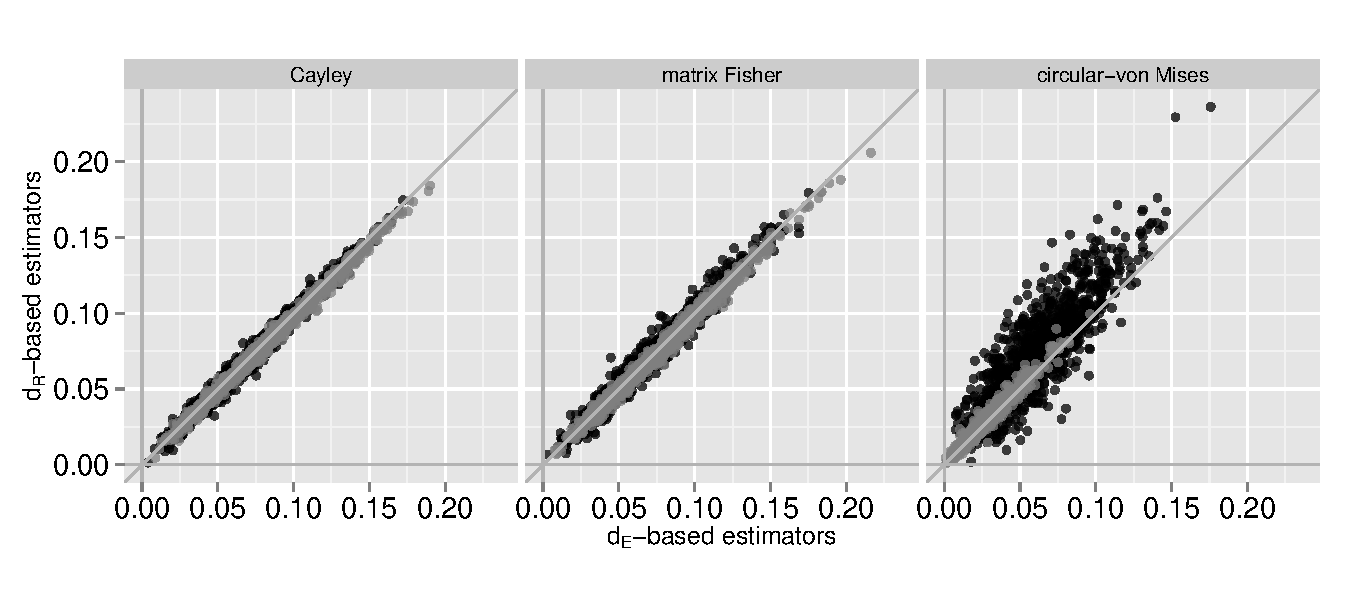
\includegraphics[width=0.8\linewidth]{EuclidRiemannNu25.pdf}}\\
%\subfloat{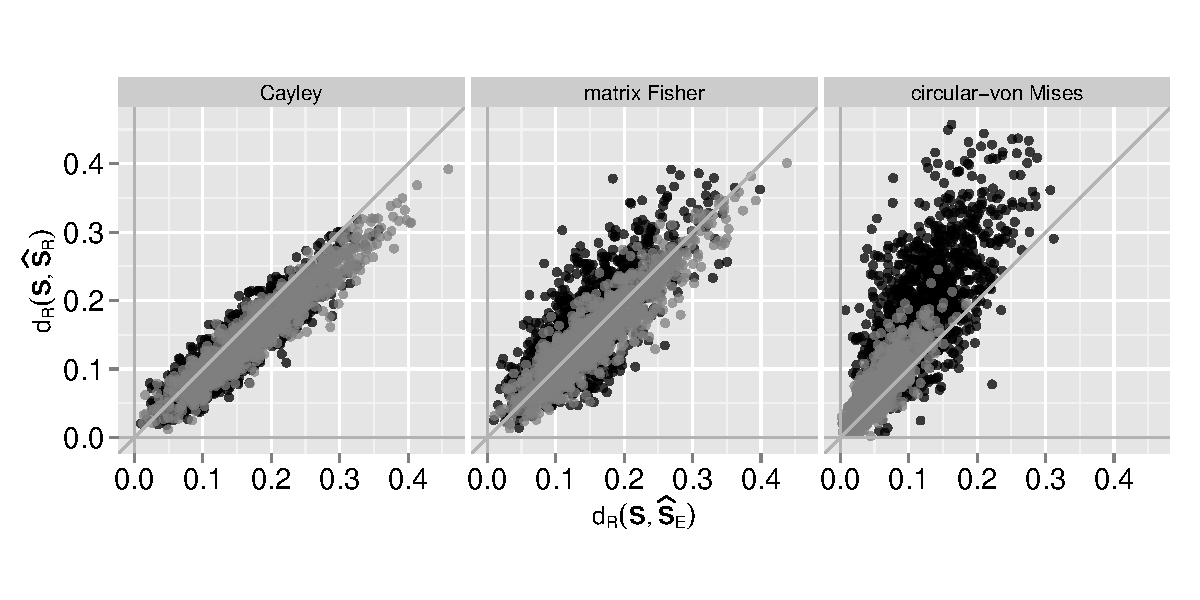
\includegraphics[width=0.8\linewidth]{EuclidRiemannNu75.pdf}}
%\caption{Comparison of the estimation errors resulting from $\Edist$ ($x$-axis) and $\Rdist$ ($y$-axis) approaches, $n=100$.  The $L_2-$norm based estimators are in black dots and the $L_1-$norm based estimators are in light gray.}
%\label{fig:comPL2}
%\end{figure}
%Tables 7 and 8 of the online supplement support Figure~\ref{fig:comPL2} with an exact count (expressed as a percentage) of how often $\Rdist$ resulted in a smaller estimation error than $\Edist$.  Additionally, we show the average amount of error by which the Riemannian $\Rdist-$ and Euclidean $\Edist-$based estimates deviate from one another.   
%Earlier results suggested the use of median-type estimators for the circular-von Mises-based distribution. Taking the findings with respect to the choice of geometry into account, we consider $\ProjMedian$ preferable for the circular-von Mises-based distribution as $\Rdist(\ProjMedian,\bm S) < \Rdist(\GeomMedian,\bm S)$ most of the time.  For the Cayley distribution our preference regarding the geometry is reversed; although differences are subtle $\Rdist$ is the preferred metric for the Cayley distribution especially when $\nu$ is large and overall $\GeomMean$ typically exhibits the least spread for this distribution.   For the  matrix Fisher distribution the preference is less clear, especially for less variable data, but as $\nu$ increases the Euclidean-based mean yields generally a smaller estimation error more often. In summary,
%\begin{itemize}
%\item the choice of location estimator can depend on the rotation error distribution in the location model (1).  For the matrix Fisher and the Cayley distribution  the projected arithmetic mean $\ProjMean$ and the geometric mean $\GeomMean$ are, respectively, preferable though $\ProjMedian$ and $\GeomMedian$ are not far behind especially when the circular spread is smaller. For the circular-von Mises-based distribution  the projected median $\ProjMedian$  should be used.
%
%\item   a significant finding of the simulation results is that the (Euclidean-based)  projected median $\ProjMedian$ is typically a good location estimator across rotation error models.  For the circular-von Mises-based estimation, this generally has the best performance, while for the Cayley or matrix Fisher distributions, this estimator is often quite comparable to the best estimator.  In other words, $\ProjMedian$, an estimator  not previously considered for rotation matrices in the literature, appears to be suggestible, particularly in small samples and without knowledge of the underlying rotation error distribution.
%
%>>>>>>> 2ae524a3512a18ca58f9808d9a1c66a11687f0c3
\end{itemize}